% ============================================================
% PATENT APPLICATION PRESENTATION
% Cross-Layer Multi-Modal Threat Detection — Patent Presentation
% Prepared for: Patent Office Evaluation
% Date: April 2026
% ============================================================

\documentclass[10pt, aspectratio=169]{beamer}

% --- Theme & Color Setup ---
\usetheme{Madrid}
\usecolortheme{whale}
\usefonttheme{professionalfonts}

% Custom color definitions
\definecolor{patentblue}{RGB}{0, 51, 102}
\definecolor{accentgold}{RGB}{191, 155, 48}
\definecolor{lightgray}{RGB}{240, 240, 240}

\setbeamercolor{palette primary}{bg=patentblue, fg=white}
\setbeamercolor{palette secondary}{bg=patentblue!80, fg=white}
\setbeamercolor{palette tertiary}{bg=patentblue!60, fg=white}
\setbeamercolor{structure}{fg=patentblue}
\setbeamercolor{title}{fg=white, bg=patentblue}
\setbeamercolor{frametitle}{fg=white, bg=patentblue}
\setbeamercolor{block title}{bg=patentblue, fg=white}
\setbeamercolor{block body}{bg=lightgray, fg=black}
\setbeamercolor{item}{fg=patentblue}
\setbeamercolor{footline}{bg=patentblue!90, fg=white}

% --- Packages ---
\usepackage[utf8]{inputenc}
\usepackage[T1]{fontenc}
\usepackage{lmodern}
\usepackage{graphicx}
\usepackage{booktabs}
\usepackage{tikz}
\usetikzlibrary{shapes.geometric, arrows.meta, positioning, calc, fit}
\usepackage{amsmath}
\usepackage{hyperref}

% --- Slide numbering in footer ---
\setbeamertemplate{navigation symbols}{}
\setbeamertemplate{footline}{%
  \leavevmode%
  \hbox{%
    \begin{beamercolorbox}[wd=.5\paperwidth,ht=2.5ex,dp=1ex,center]{footline}%
      \textbf{Patent Application — Cross-Layer Threat Detection}
    \end{beamercolorbox}%
    \begin{beamercolorbox}[wd=.5\paperwidth,ht=2.5ex,dp=1ex,right]{footline}%
      \textbf{\insertframenumber{} / \inserttotalframenumber}\hspace*{2em}
    \end{beamercolorbox}%
  }%
  \vskip0pt%
}

% --- Title Information ---
\title[Cross-Layer Threat Detection]{\textbf{System and Method for Cross-Layer\\Multi-Modal Threat Detection in\\Healthcare Environments}}
\subtitle{Patent Application Presentation}
\author{Rudra Saxena \and Rohan Sharma \and Vishal Dev Verma}
\institute{Patent Application Presentation}
\date{April 2026}

% ============================================================
\begin{document}

% ============================================================
% SLIDE 1 — Title Slide
% ============================================================
\begin{frame}[plain]
  \vfill
  \begin{center}
    {\large\textbf{\textcolor{patentblue}{System and Method for Cross-Layer Multi-Modal\\Threat Detection in Healthcare Environments}}}\\[14pt]
    {\normalsize A Privacy-Preserving\\
    Insider-Risk Platform for Critical Healthcare Infrastructure\\
    Using Edge Sensor Fusion, Hashed Behavioral Monitoring,\\
    Isolation-Forest Anomaly Detection, and Explainable Risk Scoring}\\[18pt]
    \textcolor{accentgold}{\rule{0.5\textwidth}{1pt}}\\[12pt]
    {\small\textbf{Inventors:}}\\[4pt]
    {\small Rudra Saxena (23BCE1386)}\\[2pt]
    {\small Rohan Sharma (23BCE1391)}\\[2pt]
    {\small Vishal Dev Verma (23BCE1416)}\\[10pt]
    {\small\textbf{Date:} 11 April 2026}\\[4pt]
    {\small\textbf{TRL:} 4--5 (Lab-validated, simulated hospital environment)}
  \end{center}
  \vfill
\end{frame}

% ============================================================
% SLIDE 2 — Problem Statement
% ============================================================
\begin{frame}{Problem Statement}
  \begin{block}{The Dual-Threat Challenge in Healthcare}
    Hospitals operate life-critical equipment (ventilators, infusion pumps, narcotics cabinets)
    facing \textbf{two simultaneous, uncorrelated threat classes}:
  \end{block}
  \vspace{6pt}
  \begin{columns}[T]
    \begin{column}{0.48\textwidth}
      \textbf{\textcolor{patentblue}{Physical Threats}}
      \begin{itemize}
        \item Tampering with medical devices
        \item Unauthorized cabinet access
        \item Equipment theft or displacement
        \item Environmental faults (vibration, impact)
      \end{itemize}
    \end{column}
    \begin{column}{0.48\textwidth}
      \textbf{\textcolor{patentblue}{Digital Threats}}
      \begin{itemize}
        \item Unauthorized host logins
        \item Malicious shell commands
        \item Privilege escalation attempts
        \item Insider policy violations
      \end{itemize}
    \end{column}
  \end{columns}
  \vspace{8pt}
  \begin{alertblock}{Critical Constraint}
    Transmitting raw commands and patient-adjacent data violates
    \textbf{HIPAA}, \textbf{GDPR}, and \textbf{DPDP} regulations.
  \end{alertblock}
\end{frame}

% ============================================================
% SLIDE 3 — Limitations of Existing Art
% ============================================================
\begin{frame}{Limitations of Existing Approaches}
  \begin{table}[h]
    \centering
    \small
    \begin{tabular}{@{}p{3.8cm}p{8.5cm}@{}}
      \toprule
      \textbf{Existing Technology} & \textbf{Limitation} \\
      \midrule
      Traditional EDR / Host IDS &
        Ships raw commands; no physical-world input; no healthcare context \\[4pt]
      Physical Security (CCTV, door sensors) &
        Operates in isolation from host behavior; no digital correlation \\[4pt]
      IoT Tamper Sensors &
        Local hardware alarm only; no integration with host analytics \\[4pt]
      Rule-based Insider Tools &
        Static ACLs; cannot detect legitimate credentials used in illegitimate \textit{patterns} \\[4pt]
      Generic UEBA Products &
        Rely on raw log content; not hash-based; no sensor fusion \\[4pt]
      ML-based IDS &
        Opaque scoring; clinical staff cannot interpret or act on results \\
      \bottomrule
    \end{tabular}
  \end{table}
  \vspace{4pt}
  \begin{block}{Key Gap Identified}
    \textbf{No existing solution} fuses physical + digital telemetry at the feature-vector level
    while preserving privacy and providing explainable, device-criticality-aware alerts.
  \end{block}
\end{frame}

% ============================================================
% SLIDE 4 — Proposed Solution Overview
% ============================================================
\begin{frame}{Proposed Invention}
  \textbf{A unified, cross-layer threat engine} that fuses physical and digital telemetry
  under a single anomaly model with privacy-by-construction.
  \vspace{6pt}
  \begin{columns}[T]
    \begin{column}{0.48\textwidth}
      \textbf{\textcolor{patentblue}{Core Components}}
      \begin{enumerate}
        \item \textbf{Endpoint Agent} — Linux host monitor; transmits only SHA-256 command hashes
        \item \textbf{Sensor Layer} — MPU-6050 (gyro/accel), HW-485 (sound), HW-509 (magnetic)
        \item \textbf{Detection Engine} — PSI + Isolation Forest + XAI pipeline
        \item \textbf{Web Dashboard} — Real-time alerts with explainable risk scores
      \end{enumerate}
    \end{column}
    \begin{column}{0.48\textwidth}
      \textbf{\textcolor{patentblue}{Key Differentiators}}
      \begin{itemize}
        \item Hash-only command telemetry (PSI)
        \item Cross-layer temporal fusion
        \item Device-criticality-weighted scoring
        \item Role/shift-aware insider baselining
        \item Clinician-readable XAI explanations
        \item Single engine replaces 3 vendor products
      \end{itemize}
    \end{column}
  \end{columns}
\end{frame}

% ============================================================
% SLIDE 5 — System Architecture
% ============================================================
\begin{frame}{System Architecture}
  \begin{center}
    \resizebox{0.95\textwidth}{!}{%
    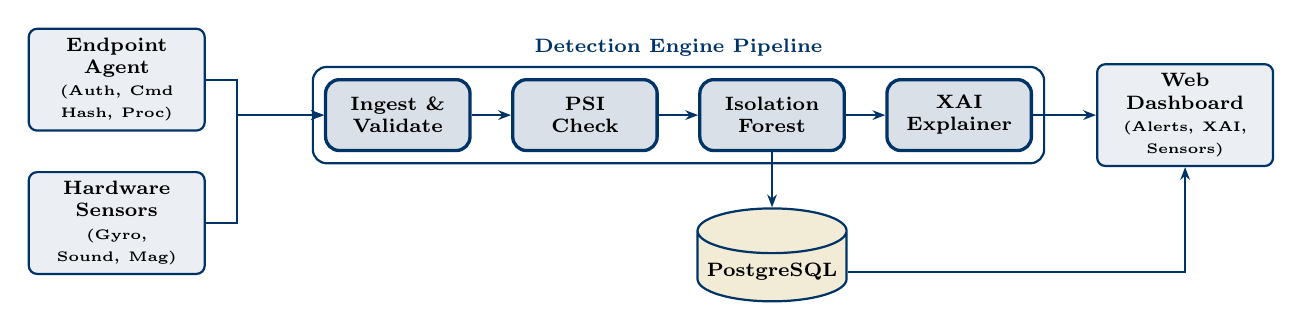
\begin{tikzpicture}[
      node distance=0.5cm and 0.8cm,
      block/.style={rectangle, draw=patentblue, fill=patentblue!8, thick,
                    rounded corners=3pt, minimum height=0.9cm, minimum width=2.2cm,
                    text width=2.0cm, align=center, font=\scriptsize\bfseries},
      engine/.style={rectangle, draw=patentblue, fill=patentblue!15, very thick,
                     rounded corners=5pt, minimum height=0.9cm, minimum width=1.8cm,
                     text width=1.6cm, align=center, font=\scriptsize\bfseries},
      db/.style={cylinder, draw=patentblue, fill=accentgold!20, thick,
                 shape border rotate=90, aspect=0.3,
                 minimum height=0.7cm, minimum width=1.2cm,
                 font=\scriptsize\bfseries},
      arr/.style={-{Stealth[scale=0.7]}, thick, patentblue}
    ]
      % Left column — data sources
      \node[block] (agent) {Endpoint\\Agent\\{\tiny (Auth, Cmd Hash, Proc)}};
      \node[block, below=0.5cm of agent] (sensors) {Hardware\\Sensors\\{\tiny (Gyro, Sound, Mag)}};

      % Center column — engine pipeline stages
      \node[engine, right=1.5cm of agent, yshift=-0.45cm] (ingest) {Ingest \&\\Validate};
      \node[engine, right=0.5cm of ingest] (psi) {PSI\\Check};
      \node[engine, right=0.5cm of psi] (ml) {Isolation\\Forest};
      \node[engine, right=0.5cm of ml] (xai) {XAI\\Explainer};

      % Engine label
      \node[draw=patentblue, thick, rounded corners=5pt,
            inner sep=4pt, fit=(ingest)(psi)(ml)(xai),
            label={[font=\scriptsize\bfseries, text=patentblue]above:Detection Engine Pipeline}] (enginebox) {};

      % Database
      \node[db, below=0.7cm of ml] (db) {PostgreSQL};

      % Dashboard
      \node[block, right=0.8cm of xai] (dash) {Web\\Dashboard\\{\tiny (Alerts, XAI, Sensors)}};

      % Arrows
      \draw[arr] (agent.east) -- ++(0.4,0) |- (ingest.west);
      \draw[arr] (sensors.east) -- ++(0.4,0) |- (ingest.west);
      \draw[arr] (ingest) -- (psi);
      \draw[arr] (psi) -- (ml);
      \draw[arr] (ml) -- (xai);
      \draw[arr] (xai) -- (dash);
      \draw[arr] (ml.south) -- (db.north);
      \draw[arr] (db.east) -| (dash.south);

    \end{tikzpicture}
    }% end resizebox
  \end{center}
  \vspace{2pt}
  \begin{itemize}\small
    \item \textbf{Privacy enforced at schema level}: \texttt{command} events carry only \texttt{command\_hash} — raw text never leaves the endpoint
    \item \textbf{Unified event schema}: All event types (\texttt{auth}, \texttt{command}, \texttt{process}, \texttt{sensor}) validated against a single JSON schema
  \end{itemize}
\end{frame}

% ============================================================
% SLIDE 6 — Inventive Step & Novelty
% ============================================================
\begin{frame}{Novelty and Inventive Step}
  \begin{block}{What Makes This Invention Non-Obvious?}
    No prior art combines all of these elements in a single system:
  \end{block}
  \vspace{4pt}
  \begin{enumerate}\small
    \item \textbf{Cross-Layer Temporal Fusion as a First-Class Feature}\\
      {\footnotesize Physical + digital events fused at the \textit{feature-vector level} before ML scoring,
      not merely concatenated at the UI level.}
    \item \textbf{Hash-Only Command Telemetry via PSI}\\
      {\footnotesize Privacy enforced structurally by the schema and hash function — not by policy.}
    \item \textbf{Device-Criticality-Weighted Risk Scoring}\\
      {\footnotesize Same anomaly scored differently on an ICU ventilator (\texttimes 2.0) vs.\ a lobby kiosk (\texttimes 1.0).}
    \item \textbf{Explainable AI for Non-ML Audiences}\\
      {\footnotesize Clinician-readable paragraphs citing both physical and digital contributors.}
    \item \textbf{Role- and Shift-Aware Insider Baselining}\\
      {\footnotesize Unsupervised behavioral envelopes per staff role — detects pattern deviations, not identity.}
    \item \textbf{Single Engine, Single Model Surface}\\
      {\footnotesize Covers outsider attacks, insider misuse, physical tampering, and device-health precursors.}
  \end{enumerate}
\end{frame}

% ============================================================
% SLIDE 7 — Cross-Layer Fusion (Key Innovation)
% ============================================================
\begin{frame}{Key Innovation: Cross-Layer Temporal Fusion}
  \begin{center}
    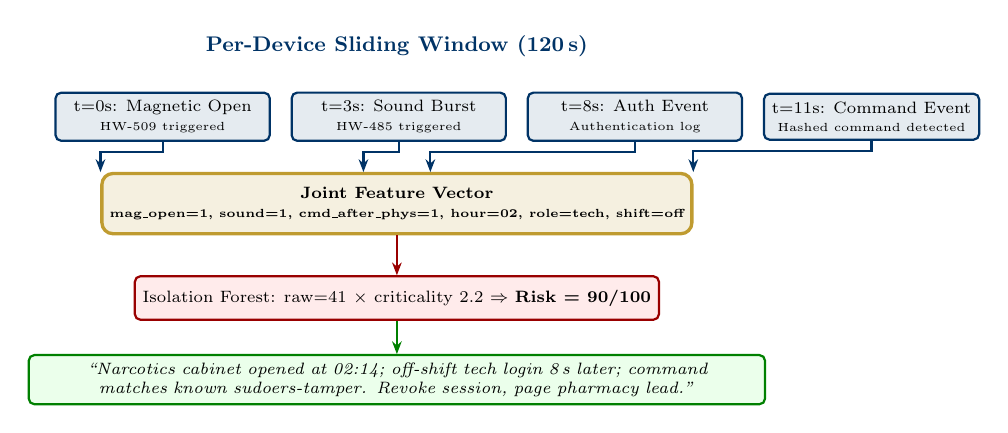
\begin{tikzpicture}[
      node distance=0.4cm,
      event/.style={rectangle, draw=patentblue, fill=patentblue!10, thick,
                    rounded corners=2pt, minimum height=0.65cm, minimum width=3.2cm,
                    align=center, font=\scriptsize},
      fusion/.style={rectangle, draw=accentgold, fill=accentgold!15, very thick,
                     rounded corners=4pt, minimum height=0.9cm, minimum width=4.0cm,
                     align=center, font=\scriptsize\bfseries},
      arr/.style={-{Stealth[scale=0.7]}, thick, patentblue},
      scale=0.85, transform shape
    ]
      % Timeline header
      \node[font=\small\bfseries, text=patentblue] (title) {Per-Device Sliding Window (120\,s)};

      % Events
      \node[event, below=0.4cm of title, xshift=-3.5cm] (e1) {t=0s: Magnetic Open\\{\tiny HW-509 triggered}};
      \node[event, right=0.3cm of e1] (e2) {t=3s: Sound Burst\\{\tiny HW-485 triggered}};
      \node[event, right=0.3cm of e2] (e3) {t=8s: Auth Event\\{\tiny Authentication log}};
      \node[event, right=0.3cm of e3] (e4) {t=11s: Command Event\\{\tiny Hashed command detected}};

      % Arrow down to fusion
      \node[fusion, below=0.8cm of title, yshift=-0.8cm] (fuse) {Joint Feature Vector\\{\tiny mag\_open=1, sound=1, cmd\_after\_phys=1, hour=02, role=tech, shift=off}};

      \draw[arr] (e1.south) -- ++(0,-0.15) -| (fuse.north west);
      \draw[arr] (e2.south) -- ++(0,-0.15) -| ([xshift=-0.5cm]fuse.north);
      \draw[arr] (e3.south) -- ++(0,-0.15) -| ([xshift=0.5cm]fuse.north);
      \draw[arr] (e4.south) -- ++(0,-0.15) -| (fuse.north east);

      % Scoring
      \node[event, below=0.6cm of fuse, fill=red!8, draw=red!60!black] (score)
        {Isolation Forest: raw=41 $\times$ criticality 2.2 $\Rightarrow$ \textbf{Risk = 90/100}};
      \draw[arr, red!60!black] (fuse.south) -- (score.north);

      % XAI
      \node[event, below=0.5cm of score, fill=green!8, draw=green!50!black, minimum width=11cm, text width=10.5cm] (xai)
        {\textit{``Narcotics cabinet opened at 02:14; off-shift tech login 8\,s later; command matches
        known sudoers-tamper. Revoke session, page pharmacy lead.''}};
      \draw[arr, green!50!black] (score.south) -- (xai.north);
    \end{tikzpicture}
  \end{center}
  \vspace{2pt}
  \begin{itemize}\small
    \item A \textbf{pure EDR} sees only a low-severity suspicious command
    \item A \textbf{pure physical alarm} sees only a routine cabinet opening
    \item \textbf{Only the fused engine} produces the correct \textbf{high-severity, actionable alert}
  \end{itemize}
\end{frame}

% ============================================================
% SLIDE 8 — Proposed Patent Claims
% ============================================================
\begin{frame}[shrink=5]{Proposed Patent Claims}
  \begin{block}{Independent Claims}
  \end{block}
  \vspace{3pt}
  \begin{description}[\textbf{Claim 3.}]\small
    \item[\textbf{Claim 1.}] \textbf{System Claim} — A healthcare threat-detection system comprising a Linux endpoint
      agent transmitting only normalized SHA-256 command hashes, physical sensors
      (MEMS inertial + acoustic + magnetic), and a detection engine with unified event schema.
    \item[\textbf{Claim 2.}] \textbf{Method Claim} — A method of detecting cross-layer threats by:
      (i)~collecting hashed behavioral events, (ii)~collecting physical sensor events,
      (iii)~fusing within a temporal window, (iv)~scoring with device-criticality-weighted
      Isolation Forest, (v)~producing human-readable explanation.
    \item[\textbf{Claim 3.}] \textbf{CRM Claim} — A non-transitory computer-readable medium storing
      instructions to perform the method of Claim~2.
  \end{description}
  \vspace{3pt}
  \begin{block}{Key Dependent Claims}
  \end{block}
  \vspace{3pt}
  \begin{description}[\textbf{Claim 8.}]\small
    \item[\textbf{Claim 4.}] Per-device temporal fusion window with joint feature vectors
    \item[\textbf{Claim 5.}] PSI-style set-membership test over SHA-256 hashes
    \item[\textbf{Claim 6.}] XAI module generating natural-language justifications
    \item[\textbf{Claim 7.}] Role/shift-aware insider-risk baselining
    \item[\textbf{Claim 8.}] Federated multi-hospital deployment sharing only model parameters
  \end{description}
\end{frame}

% ============================================================
% SLIDE 9 — Advantages & Market Potential
% ============================================================
\begin{frame}{Advantages and Market Potential}
  \begin{columns}[T]
    \begin{column}{0.52\textwidth}
      \textbf{\textcolor{patentblue}{Advantages Over Prior Art}}
      \begin{itemize}\small
        \item \textbf{Privacy by construction} — HIPAA/GDPR/DPDP compliant; raw commands never leave endpoint
        \item \textbf{Lower false-positive rate} — cross-layer context suppresses benign-looking anomalies
        \item \textbf{Higher detection of subtle attacks} — catches multi-step physical $\rightarrow$ digital chains
        \item \textbf{Criticality-aware triage} — ICU ventilator alerts surface above lobby printer alerts
        \item \textbf{Actionable XAI} — reduces mean time to action without needing a data scientist
        \item \textbf{Low cost} — commodity sensors (\$5--15 each), open-source software stack
        \item \textbf{Replaces 3 vendor products} with one unified platform
      \end{itemize}
    \end{column}
    \begin{column}{0.44\textwidth}
      \textbf{\textcolor{patentblue}{Healthcare Cybersecurity Market}}\\[4pt]
      \begin{table}
        \centering
        \footnotesize
        \begin{tabular}{@{}cr@{}}
          \toprule
          \textbf{Year} & \textbf{Market Size} \\
          \midrule
          2024 & \raise.17ex\hbox{$\scriptstyle\sim$}USD 20\,B \\
          2026 & \raise.17ex\hbox{$\scriptstyle\sim$}USD 27\,B \\
          2028 & \raise.17ex\hbox{$\scriptstyle\sim$}USD 38\,B \\
          2030 & \raise.17ex\hbox{$\scriptstyle\sim$}USD 52\,B \\
          \bottomrule
        \end{tabular}
      \end{table}
      \vspace{4pt}
      {\footnotesize\textbf{Growth drivers:}
      \begin{itemize}\scriptsize
        \item Hospital ransomware surge
        \item FDA pre-market cyber requirements
        \item EU MDR, HIPAA enforcement
        \item Hospital IoT proliferation
        \item AI-driven security adoption
      \end{itemize}}
    \end{column}
  \end{columns}
\end{frame}

% ============================================================
% SLIDE 10 — Summary & Conclusion
% ============================================================
\begin{frame}{Summary and Conclusion}
  \begin{block}{Invention Summary}
    The proposed system is the first cross-layer, privacy-preserving,
    explainable threat-detection platform purpose-built for healthcare infrastructure.
  \end{block}
  \vspace{6pt}
  \begin{columns}[T]
    \begin{column}{0.48\textwidth}
      \textbf{\textcolor{patentblue}{Patentability Criteria Met}}
      \begin{itemize}\small
        \item[\checkmark] \textbf{Novelty} — No prior art combines hash-only PSI + sensor fusion + Isolation Forest + XAI + insider baselining
        \item[\checkmark] \textbf{Inventive Step} — Cross-domain insight required (cybersecurity + IoT + ML + clinical workflow)
        \item[\checkmark] \textbf{Industrial Applicability} — Validated at TRL 4--5; commodity hardware; clear path to deployment
      \end{itemize}
    \end{column}
    \begin{column}{0.48\textwidth}
      \textbf{\textcolor{patentblue}{Next Steps}}
      \begin{itemize}\small
        \item Clinical pilot in an operational hospital ward (TRL 6)
        \item Independent red-team tamper exercises
        \item Quantitative evaluation: expected \textbf{+18--25\% F1} improvement from fusion
        \item Federated multi-hospital validation
        \item Filing of provisional patent application
      \end{itemize}
    \end{column}
  \end{columns}
  \vspace{10pt}
  \begin{center}
    \textcolor{accentgold}{\rule{0.4\textwidth}{1pt}}
  \end{center}
\end{frame}

\end{document}
